\subsection{Đề 2}
\Opensolutionfile{ans}[ans/ans-2-B2-De2-lc]
\caulc
\begin{ex}%[2D1N3-1]
	Cho hàm số $y=f(x)$ liên tục trên $[-3 ; 2]$ và có bảng biến thiên như hình dưới đây. Gọi $M$ và $m$ lần lượt là giá trị lớn nhất và giá trị nhỏ nhất của hàm số $y=f(x)$ trên $[-1 ; 2]$.
	\begin{center}
		
\begin{tikzpicture}
			\tkzTabInit[nocadre=false,lgt=0.7,espcl=2.1,deltacl=0.5]
			{$x$ /0.7,$y'$ /0.7,$y$ /2}
			{$-3$,$-1$,$0$,$1$,$2$}
			\tkzTabLine{,+,$0$,-,$0$,+,$0$,-,}
			\tkzTabVar{-/$2$,+/$3$,-/$0$,+/$2$,-/$1$}
		\end{tikzpicture}
	\end{center}
	Giá trị của $5M-2m$ bằng bao nhiêu?
	\choice
	{\True $15$}
	{$3$}
	{$17$}
	{$-15$}
	\loigiai{
		Ta có $M=\max \limits_{[-1 ; 2]} f(x)=f(-1)=3$ và $m=\min\limits _{[-1 ; 2]} f(x)=f(0)=0$.\\
		Vậy $5M-2m=15$.
	}
\end{ex}

\begin{ex}%[2D1N3-1]
	Giá trị nhỏ nhất của hàm số $f(x)=\dfrac{x^2+3}{x-1}$ trên đoạn $[2 ; 4]$ là
	\choice 
	{$7$}
	{\True $6$}
	{$\dfrac{19}{3}$}
	{$\dfrac{13}{3}$}
	\loigiai{
		Xét hàm số $f(x)=\dfrac{x^2+3}{x-1}$ trên $[2 ; 4]$, có $f'(x)=\dfrac{x^2-2 x-3}{(x-1)^2}$\\
		Phương trình $f'(x)=0 \Leftrightarrow $ $\heva{&2 \leq x \leq 4 \\ & x^2-2x-3=0 }$
		$ \Leftrightarrow x=3.$\\
		Tính $f(2)=7 ; f(3)=6 ; f(4)=\dfrac{19}{3}  $.\\
		Vậy $\min\limits _{[2 ; 4]} f(x)=f(3)=6  $.
	}
\end{ex}
\begin{ex}%[2D1N3-1]
	Gọi $M, m$ lần lượt là giá trị lớn nhất, giá trị nhỏ nhất của hàm số $f(x)=\dfrac{3 x-1}{x-3}$ trên đoạn $[0 ; 2]$.
	Giá trị của $3 M+m$ bằng
	\choice 
	{$0$}
	{$-4$}
	{\True $-2$}
	{$1$}
	\loigiai{Xét hàm số $f(x)=\dfrac{3 x-1}{x-3}$ trên $[0 ; 2]$         có $f'(x)=-\dfrac{8}{(x-3)^2}<0$.\\
		Suy ra $f(x)$ là hàm số nghịch biến trên $(0 ; 2) \Rightarrow \heva{& \min\limits _{[0 ; 2]} f(x)=f(2)=-5 \\& \max\limits _{[0 ; 2]} f(x)=f(0)=\dfrac{1}{3}.}$\\
		Vậy $M=\dfrac{1}{3} \Rightarrow 3 M=3 ; m=-5 \Rightarrow 3 M+m=-2$.
	}
\end{ex}
\begin{ex}%[2D1N3-1]
	Gọi $M$ và $m$ lần lượt là giá trị lớn nhất và giá trị nhỏ nhất của hàm số $y=\sqrt{1-x}+\sqrt{1+x}$. Giá trị của $M-2 m^2$ bằng
	\choice
	{\True $-2$}
	{$2$}
	{$0$}
	{$-1$}
	\loigiai{Điều kiện xác định $\heva{&1-x \geq 0  \\& x+1 \geq 0} \Leftrightarrow-1 \leq x \leq              1$.\\
		Xét hàm số $f(x)=\sqrt{1-x}+\sqrt{1+x}$ trên $[-1 ; 1]$, có $f'(x)=-\dfrac{1}{2 \sqrt{1-x}}+\dfrac{1}{2 \sqrt{1+x}}$;\\
		Phương trình $f'(x)=0 \Leftrightarrow \heva{&-1<x<1 \\& \sqrt{1-x}=\sqrt{1-x}} \Leftrightarrow x=0 $. \\
		Tính $f(-1)=f(1)=\sqrt{2} ; f(0)=2$.\\
		Vậy $\heva{&m=\min\limits _{[-1 ; 1]} f(x)=\sqrt{2} \\& M=\max \limits_{[-1 ; 1]} f(x)=2}\rightarrow M-2 m^2=2-2\cdot2=-2$.
	}
\end{ex}

\begin{ex}%[2D1H3-1]
	Giá trị nhỏ nhất của hàm số $y=2 \cos ^3 x-\dfrac{9}{2} \cos ^2 x+3 \cos x+\dfrac{1}{2}$ là
	\choice
	{$-9$}
	{\True $1$} 
	{$-\dfrac{3}{2}$}
	{$\dfrac{1}{2}$}
	\loigiai{Đặt $t=\cos x \in[-1 ; 1]$, khi đó $y=f(t)=2 t^3-\dfrac{9}{2} t^2+3 t+\dfrac{1}{2}, -1 \leq t \leq 1$.\\
		Xét hàm số $f(t)=2 t^3-\dfrac{9}{2} t^2+3 t+\dfrac{1}{2}$ trên $[-1 ; 1]$, có $f'(t)=8 t^2-9 t+3>0, \forall t\in[-1 ; 1]$.\\
		Suy ra $f(t)$ là hàm số đồng biến trên $(-1 ; 1) \Rightarrow \min \limits _{[-1 ; 1]} f(t)=f(-1)=1.$
	}
\end{ex}
\begin{ex}%[2D1N3-2]
	Giá trị lớn nhất của hàm số $y=-x^3+3 x+1$ trên khoảng $(0 ;+\infty)$ bằng
	\choice 
	{$1$}
	{\True $3$}
	{$-1$}
	{$5$}
	\loigiai{Ta có $y'=-3 x^2+3$,  $y'=0         \Leftrightarrow \heva{&x=1\in(0 ;+\infty) \\&x=-1 \notin(0 ;+\infty)}$.\\
		Bảng biến thiên
		\begin{center}
			
\begin{tikzpicture}
				\tkzTabInit[nocadre=false,lgt=0.7,espcl=2.5,deltacl=0.5]
				{$x$ /0.7,$y'$ /0.7,$y$ /2}
				{$0$,$1$,$+\infty$}
				\tkzTabLine{,+,$0$,-,}
				\tkzTabVar{-/$1$,+/$3$,-/$-\infty$}
			\end{tikzpicture}
		\end{center}
		Từ bảng biến thiên ta thấy giá trị lớn nhất của hàm số $y=-x^3+3 x+1$ trên khoảng $(0 ;+\infty)$ bằng 3.}
\end{ex}
\begin{ex}%[2D1N3-1]
	Cho hàm số $y=f(x)$ có đồ thị như hình vẽ. Gọi $m$ và $M$ lần lượt là giá trị nhỏ nhất và giá trị lớn nhất của hàm số $f(x)$ trên đoạn $[-1 ; 1]$. 
	\begin{center}
		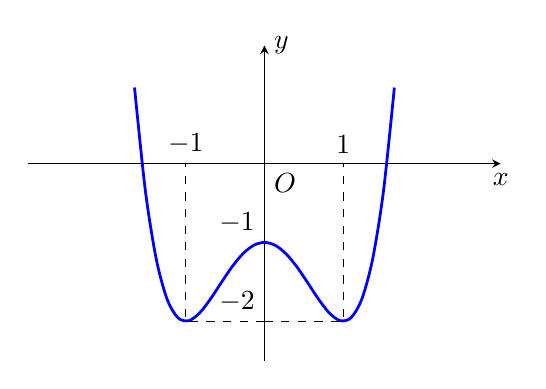
\begin{tikzpicture}[>=stealth]
			\draw[->] (-3,0) --(0,0) node[below
			right]{$O$} -- (3,0)
			node[below]{$x$};
			\draw[->](0,-2.5)--(0,1.5)
			node[right]{$y$};
			\draw[smooth,blue,line width=1]
			plot[domain=-1.65:1.65]
			(\x,{(\x)^(4)-2*(\x)^(2)-1});
			\draw[dashed] (0,-2)
			node[left]{} -- (1,-2) --
			(1,0) node[above]{$1$};
			\draw[dashed] (0,-2)
			node[above left]{$-2$} -- (-1,-2) --
			(-1,0) node[above]{$-1$};
			\draw (0,-1) node[above left] {$-1$};	
		\end{tikzpicture}
	\end{center}
	Khẳng định nào sau đây là đúng?
	\choice 
	{$m+M=2$}
	{$m+M=-2$}
	{$m+M=0$}
	{\True $m+M=-3$}
	\loigiai{
		Dựa vào đồ thị, ta thấy trên đoạn $[-1 ; 1]$, hàm số đạt:\\
		Giá trị lớn nhất $M=-1$ tại $x=0$.\\
		Giá trị nhỏ nhất $m=-2$ tại $x= \pm1$.\\
		Suy ra $m+M=-3$.}
\end{ex}
\begin{ex}%[2D1H3-1]
	Tìm giá trị thực của tham số $a$ để hàm số $f(x)=-x^3-3 x^2+a$ có giá trị nhỏ nhất trên đoạn $[-1 ; 1]$ bằng 0.
	\choice  
	{$a=2$}
	{$a=6$}
	{$a=0$}
	{\True $a=4$}
	\loigiai{Xét hàm số $f(x)=-x^3-3 x^2+a$ trên $[-1 ; 1]$, có   $f'(x)=-3 x^2-6 x.$\\
		Phương trình $f'(x)=0 \Leftrightarrow \heva{&-1 \leq x \leq 1 \\& -3 x^2-6 x=0} \Rightarrow x=0$.\\
		Tính $f(-1)=-2+a ; f(0)=a ; f(1)=-4+a.$\\
		Suy ra $\min \limits_{[-1: 1]} f(x)=f(1)=-4+a=0 \Rightarrow a=4$. 
	}
\end{ex}
\begin{ex}%[2D1H3-3]
	Cho hàm số $y=f(x)$ liên tục trên $\mathbb{R}$ và có đồ thị như hình dưới
	\begin{center}
		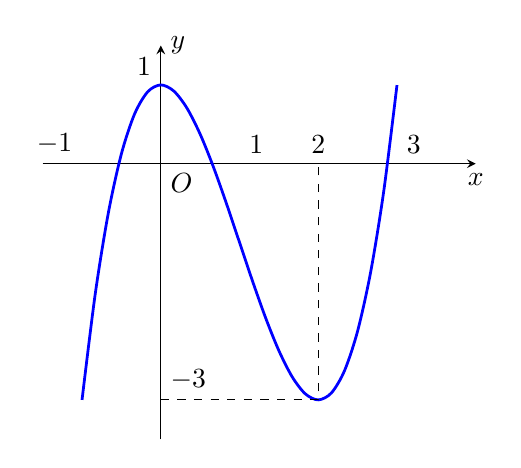
\begin{tikzpicture}[>=stealth]
			\draw[->] (-1.5,0) --(0,0) node[below
			right]{$O$} -- (4,0)
			node[below]{$x$};
			\draw[->](0,-3.5)--(0,1.5)
			node[right]{$y$};
			\draw[smooth,blue,line width=1]
			plot[domain=-1:3]
			(\x,{(\x)^(3)-3*(\x)^(2)+1});
			\draw[dashed] (0,-3) node[left]{} -- (2,-3) --
			(2,0) node[above]{$2$};
			\draw (0,-3) node[above right] {$-3$};
			\draw (1,0) node[above right] {$1$};
			\draw (0,1) node[above left] {$1$};	
			\draw (3,0) node[above right] {$3$};	
			\draw (-1,0) node[above left] {$-1$};	
		\end{tikzpicture}
	\end{center}
	Tìm giá trị lớn nhất của hàm số $y=f^2(x)+3$ trên đoạn $[0 ; 2]$.
	\choice 
	{\True $12$}
	{$13$}
	{$2$}
	{$9$}
	\loigiai{
		Đặt $g(x)=f^2(x)+3$. Từ đồ thị đã cho ta có $\exists x_0 \in(0 ; 1)$ để $f\left(x_0\right)=0$.
		$$
		\begin{gathered}
			\text { Và } \forall x \in[0 ; 2] \text { thì }-3 \leq f(x) \leq 1 \Rightarrow 0 \leq f^2(x) \leq 9 \Rightarrow 3 \leq f^2(x)+3 \leq 12 \Rightarrow 3 \leq g(x) \leq 12 \\
			\Rightarrow \max _{[0 ; 2]} g(x)=12 \text { khi } f(x)=-3 \Leftrightarrow x=2 \in[0 ; 2] .
		\end{gathered}
		$$}
\end{ex}
\begin{ex}%[2D1V3-1]
	Cho hàm số $f(x)=\dfrac{x-m^2}{x+8}$ với $m$ là tham số thực. Tìm giá trị lớn nhất của $m$ để hàm số có giá trị nhỏ nhất trên đoạn $[0 ; 3]$ bằng -2.
	\choice  
	{$m=-4$}
	{$m=5$}
	{\True $m=4$}
	{$m=1$}
	\loigiai{
		Xét hàm số $f(x)=\dfrac{x-m^2}{x+8}$ trên $[0 ; 3]$, có $f'(x)=\dfrac{8+m^2}{(x+8)^2}>0 , \forall x \in[0 ; 3]$\\
		Suy ra $f(x)$ là hàm số đồng biến trên $(0 ; 3) \Rightarrow \min \limits _{[0 ; 3]} f(x)=f(0)=-\dfrac{m^2}{8}$\\
		Theo bài ta, ta có $\min \limits _{[0 ; 3]} f(x)=-2 \Leftrightarrow-\dfrac{m^2}{8}=-2 \Leftrightarrow m^2=16 \Rightarrow m_{\max }=4$.
	}
\end{ex}
\begin{ex}%[2D1V3-1]
	Cho hàm số $f(x)$ có đạo hàm $f'(x)=(x+1)(x-1)^2(x-2)$. Giá trị nhỏ nhất của hàm số $g(x)=f(x)+\dfrac{1}{3} x^3-x-2$ trên đoạn $[-1 ; 2]$ bằng
	\choice 
	{$f(2)-\dfrac{4}{3}$}
	{\True $f(1)-\dfrac{8}{3}$}
	{$f(0)-2$}
	{$f(-1)-\dfrac{4}{3}$}
	\loigiai{
		Ta có $g'(x)=f'(x)+x^2-1$.\\
		Khi đó $g'(x)=0 \Leftrightarrow(x+1)(x-1)^2(x-2)+x^2-1=0 \\
		\Leftrightarrow\left(x^2-1\right)\left(x^2-3 x+3\right)=0 \Leftrightarrow x= \pm 1$.\\
		Do phương trình $x^2-3 x+3=0$ vô nghiệm.\\
		Bảng biến thiên
		\begin{center}
			
\begin{tikzpicture}
				\tkzTabInit[nocadre=false,lgt=1.5,espcl=2.1,deltacl=0.7]
				{$x$ /0.7,$g'(x)$ /0.7,$g(x)$ /2}
				{$-1$,$1$,$2$}
				\tkzTabLine{,-,$0$,+,}
				\tkzTabVar{+/$ $,-/$g(1)$,+/$ $}
			\end{tikzpicture}
		\end{center}
		Hàm số đạt giá trị nhỏ nhất tại $x=1$ và GTNN bằng $g(1)=f(1)-\dfrac{8}{3}$.}
\end{ex}
\begin{ex}%[2D1V3-1]
	Hỏi tập hợp nào dưới đây chứa tất cả các giá trị thực của tham số $m$ để giá trị lớn nhất của hàm số $y=\left|x^4-2 x^2+m\right|$ trên đoạn $[0 ; 2]$ bằng $5$?
	\choice  
	{$(-\infty ;-5) \cup(0 ;+\infty)  $}
	{\True $(-5 ;-2)  $}
	{$(-4 ;-1) \cup(5 ;+\infty)  $}
	{$(-4 ;-3)  $}
	\loigiai{
		Xét hàm số $f(x)=x^4-2 x^2+m$ trên $[0 ; 2]$.\\
		Ta có $f'(x)=4 x^3-4 x$; $ f'(x)=0\Leftrightarrow 
		\hoac{&x=0 \\& x= \pm 1}$\\
		Tính $|f(0)|=|m| ;  |f(1)|=|m-1| ;   |f(2)|=|m+8|$.\\
		Suy ra $\max  \limits_{[1 ; 2]} y=\{|m-1| ;|m+8|\}$
		\begin{itemize}
			\item  Nếu $\max \limits _{[1 ; 2]} y=|m-1| \text{ thì } \heva{|m-1|=5 \\ |m-1| \geq|m+8|} \Leftrightarrow m=-4 $.\\
			\item Nếu $\max \limits _{[1 ; 2]} y=|m+8| \text{ thì } \heva{|m+8|=5 \\ |m+8| \geq|m-1|}\Leftrightarrow m=-3$.\\
		\end{itemize}
		Vậy có 2 giá trị $m$ cần tìm và thuộc khoảng $(-5 ;-2)  $.} 
\end{ex}
\Closesolutionfile{ans}
\indapan{6}{ans/ans-2-B2-De2-lc}
\Opensolutionfile{ans}[ans/ans-2-B2-De2-ds]
\cauds
\setcounter{ex}{0}
\begin{ex}%[2D1N3-1]
	Cho hàm số $y=f(x)$ xác định trên tập  $\mathscr{D}$. Số $M$ và $m$ lần lượt được gọi là giá trị lớn nhất và giá trị nhỏ nhất của hàm số $y=f(x)$ trên  $\mathscr{D}$.
	\choiceTF
	{$f(x) \geq M$ với mọi $x \in \mathscr{D}$ thì M là GTLN của hàm số}
	{\True $m$ là GTNN nếu $f(x)\geq  m$ với mọi $x \in  \mathscr{D}$ và tồn tại $x_0 \in \mathscr{D}$ sao cho $f\left(x_0\right)=m$}
	{$M-m=0$}
	{\True $M$ là GTLN nếu $f(x)\leq M$ với mọi $x \in \mathscr{D}$ và tồn tại $x_0 \in \mathscr{D}$ sao cho $f\left(x_0\right)=M$}
	\loigiai{    
		\begin{itemchoice}
			\itemch Sai. $M$ là GTLN nếu $f(x) \leq M$ với mọi $x \in \mathscr{D}$ và tồn tại $x_0 \in \mathscr{D}$ sao cho $f\left(x_0\right)=M$.
			\itemch Đúng. Số $m$ được gọi là GTNN của hàm số $y=f(x)$ trên $\mathscr{D}$ nếu $f(x) \geq m$ với mọi $x \in \mathscr{D}$ và tồn tại $x_0 \in \mathscr{D}$ sao cho $f\left(x_0\right)=m$. 
			\itemch Sai.
			\itemch Đúng.  Số $M$ được gọi là GTLN của hàm số $y=f(x)$ trên $\mathscr{D}$ nếu $f(x)\leq M$ với mọi $x \in \mathscr{D}$ và tồn tại $x_0 \in \mathscr{D}$ sao cho $f\left(x_0\right)=M$.
		\end{itemchoice}
	}
\end{ex}
\begin{ex}%[2D1H3-1]
	Hàm số $y=f(x)$ liên tục trên đoạn $[-2;1]$ và có hình vẽ như sau.
	\begin{center}
		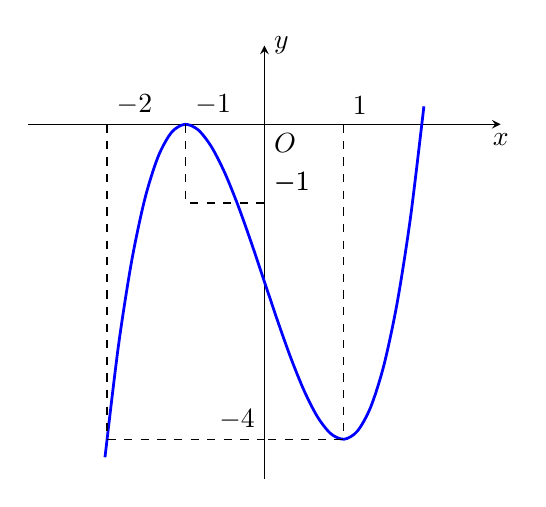
\begin{tikzpicture}[>=stealth]
			\draw[->] (-3,0) --(0,0) node[below
			right]{$O$} -- (3,0)
			node[below]{$x$};
			\draw[->](0,-4.5)--(0,1)
			node[right]{$y$};
			\draw[smooth,blue,line width=1]
			plot[domain=-2.025:2.025]
			(\x,{(\x)^(3)-3*(\x)-2});
			\draw[dashed] (-1,0)
			node[left][above right]{$-1$} -- (-1,-1) --
			(0,-1) node[above]{};
			\draw[dashed] (-2,0)
			node[above right]{$-2$} -- (-2,-4) --
			(0,-4) node[above left]{$-4$};
			\draw (0,-1) node[above right] {$-1$};
			\draw[dashed] (1,0)
			node[above right]{$1$} -- (1,-4) --
			(0,-4) node[above]{};
			\draw (0,-1) node[above right] {$-1$};
		\end{tikzpicture}
	\end{center}
	Gọi $M$ và $m$ lần lượt là GTLN và GTNN của hàm số trên $[-2;1]$.  Xét tính đúng sai trong các khẳng định sau
	\choiceTF
	{\True $m=-4$}
	{$M=-1$}
	{\True $M+m=-4$}
	{\True Hàm số đạt GTLN tại $x=-1$}
	\loigiai{
		\begin{itemchoice}
			\itemch Đúng. GTNN của hàm số trên $[-2;1]$ bằng $-4$.
			\itemch Sai.  GTLN của hàm số trên $[-2;1]$ bằng $0$.
			\itemch Đúng. $M+m=-4+0=-4$.
			\itemch Đúng. GTLN của hàm số trên $[-2;1]$ bằng $0$ tại $x=-1$.
		\end{itemchoice}
	}
\end{ex}
\begin{ex}%[2D1V3-1]
	Hàm số $y=\dfrac{x-m^2}{x+1}$. Xét trên đoạn $[-4 ;-2]$ thì
	\choiceTF 
	{\True $\min\limits _{[-4 ;-2]} y=\dfrac{4}{3}+\dfrac{m^2}{3}$}
	{$\max\limits _{[-4 ;-2]} y=2-m^2$}
	{$\min\limits_{[-4 ;-2]} y=\dfrac{3}{4}-m^2$}
	{\True $\max \limits _{[-4 ;-2]} y=2+m^2$}
	\loigiai{
		Tập xác định $\mathscr{D}=\mathbb{R} \backslash\{-1\}$.\\
		Ta có $y'=\dfrac{1+m^2}{(x+1)^2}>0, \forall x \neq-1$.\\
		Suy ra hàm số $y=\dfrac{x-m^2}{x+1}$ đồng biến trên $(-\infty ;-1) \text{ và } (-1 ;+\infty)$.\\
		Do đó $\max \limits _{[-4 ;-2]} y=y(-2)=\dfrac{-2-m^2}{-2+1}=2+m^2$.\\
		$\min \limits _{[-4 ;-2]} y=y(-4)=\dfrac{-4-m^2}{-4+1}=\dfrac{4}{3}+\dfrac{m^2}{3}$.\\
		\begin{itemchoice}
			\itemch Đúng. 
			\itemch Sai. Vì $\max \limits _{[-4 ;-2]} y=2+m^2$.
			\itemch Sai. Vì $\min \limits _{[-4 ;-2]} y=\dfrac{4}{3}+\dfrac{m^2}{3}$.
			\itemch Đúng. 
		\end{itemchoice}
	}
\end{ex}
\begin{ex}%[2D1H3-1]
	Hàm số $y=f(x)$ liên tục trên đoạn $\mathbb{R}$ và có bảng biến thiên như sau. Gọi $M$ và $m$ lần lượt là GTLN và GTNN của hàm số.  Khi đó
	\begin{center}
		
\begin{tikzpicture}
			\tkzTabInit[nocadre,lgt=1.5,espcl=2,deltacl=.5]
			{$x$/0.8, $y’$/0.8, $y$/2}
			{$-\infty$,$-1$,$0$,$\frac{1}{2}$,$+\infty$}
			\tkzTabLine{,-,0,+,0,+,0,+}
			\tkzTabVar{+/$+\infty$ ,-/ $1$,R,R ,+/$+\infty$}
		\end{tikzpicture}
	\end{center}
	\choiceTF 
	{\True $m=1$}
	{$M=+\infty$}
	{\True Hàm số không có giá trị lớn nhất}
	{$m=1$ tại $x=1$}
	\loigiai{
		\begin{itemchoice}
			\itemch Đúng. Dựa vào BBT ta có GTNN của hàm số là $m=1$.
			\itemch Sai. Không tồn tại $x_0$ thỏa mãn $f\left(x_0\right)=M$.
			\itemch Đúng. 
			\itemch Sai. GTNN của hàm số là $m=1$ tại $x=-1$.
		\end{itemchoice}
	}
\end{ex}
\Closesolutionfile{ans}
\indapan{3}{ans/ans-2-B2-De2-ds}
\Opensolutionfile{ans}[ans/ans-2-B2-De2-kq]
\caukq
\setcounter{ex}{0}
\begin{ex}%[2D1H3-1]
	Gọi $m$ và $M$ lần lượt là giá trị nhỏ nhất và giá trị lớn nhất của hàm số $y=\dfrac{1}{2} x-\sqrt{x+2}$ trên đoạn $[-1 ; 34]$. Tổng $S=3m+M$ bằng
	\shortans{$6,5$}
	\loigiai{
		Ta có $y'=\dfrac{1}{2}-\dfrac{1}{2\sqrt{x+2}}=\dfrac{\sqrt{x+2}-1}{2 \sqrt{x+2}}$.\\ 
		$y'=0 \Leftrightarrow \sqrt{x+2}=1 \Leftrightarrow x=-1 \in [-1 ; 34]$\\
		$f(-1)=-\dfrac{3}{2} ; f(34)=11 $\\
		Vậy $m=-\dfrac{3}{2} ; M=11 \Rightarrow S=3\left(-\dfrac{3}{2}\right)+11=\dfrac{-9}{2}+11=\dfrac{13}{2}=6{,}5$.
	} 
\end{ex}
\begin{ex} %[2D1V3-1]
	Cho hàm số $y=(x+m)^3-3(x+m)+1+n$. Biết hàm số nghịch biến trên khoảng $(0 ; 2)$ và giá trị lớn nhất của hàm số trên $[-1 ; 1]$ bằng 4. Tính $m+n$.
	\shortans{$0$}
	\loigiai{
		$$\begin{aligned}
			& y'=3(x+m)^2-3=3(x+m+1)(x+m-1) \\
			& y'=0 \Leftrightarrow \hoac{&x=1-m=x_2 \\ &x=-1-m=x_1.}
		\end{aligned}$$
		Để hàm số nghịch biến trên $(0 ; 2)$ thì \\
		$\heva{
			&3 \cdot y ^ { \prime } ( 0 ) \leq 0 \\
			&3 \cdot y ^ { \prime } ( 2 ) \leq 0 }
		\Leftrightarrow 
		\heva{
			& y ^ { \prime } ( 0 ) \leq 0  \\
			& y ^ { \prime } ( 2 ) \leq 0 }
		\Leftrightarrow 
		\heva{ 
			&3 m ^ { 2 } - 3 \leq 0  \\
			& 3 ( 2 + m ) ^ { 2 } - 3 \leq 0 }
		\Leftrightarrow 
		\heva{
			& m^2-1 \leq 0 \\
			& (2+m)^2-1 \leq 0}\\
		\Leftrightarrow
		\heva{
			& - 1 \leq m \leq 1  \\
			& - 1 \leq 2 + m \leq 1 }
		\Leftrightarrow 
		\heva{
			& -1 \leq m \leq 1 \\
			& -3 \leq m \leq-1}
		\Leftrightarrow 
		m=-1.$\\
		Với $m=-1$ thì $y'=0 \Leftrightarrow \hoac{&x=0 \in[-1 ; 1] \\ &x=2 \notin[-1 ; 1].}$\\
		Ta có $y(0)=n+3, y(1)=n+1, y(-1)=n-1 \Rightarrow \max \limits _{[-1 ; 1]} y=n+3=4 \Rightarrow n=1.$\\
		$\Rightarrow m+n=0$.
	} 
\end{ex}
\begin{ex} %[2D1V3-1]
	Cho hàm số $y=\left(-x^3+3 x-m-1\right)^2$. Tính tổng tất cả các giá trị của tham số $m$ sao cho giá trị nhỏ nhất của hàm số trên đoạn $[-1 ; 1]$ bằng $4$.
	\shortans{$-2$}
	\loigiai{
		Đặt $t=g(x)=-x^3+3x-1$, hàm số có bảng biến thiên như sau
		\begin{center}
			
\begin{tikzpicture}
				\tkzTabInit[nocadre,lgt=1.5,espcl=2,deltacl=.5]
				{$x$/0.5, $g’$/0.5, $g$/2}
				{$-\infty$,$-1$,$1$,$+\infty$}
				\tkzTabLine{,-,0,+,0,-,}
				\tkzTabVar{+/$+\infty$ ,-/$-3$,+/$1$,-/$-\infty$}
			\end{tikzpicture}
		\end{center}
		Từ bảng biến thiên ta thấy $x \in[-1 ; 1]$ thì $t \in[-3 ; 1]$\\
		Bài toán trở thành: Tìm $m$ để hàm số $y=f(t)=(t-m)^2$ có giá trị nhỏ nhất của hàm số trên đoạn $[-3 ; 1]$ bằng 4 .\\
		Ta có $f'(t)=2(t-m)=0 \Leftrightarrow t=m$.\\
		Nếu $m \in[-3 ; 1]$ thì $\min \limits _{[-3 ; 1]} f(t)=f(m)=0$, tức là không tồn tại $m$ thỏa mãn yêu cầu bài toán.\\
		Nếu $m>1$ thì $\min \limits _{[-3 ; 1]} f(t)=f(1)=(1-m)^2 \Leftrightarrow(1-m)^2=4 \Leftrightarrow \hoac{&m=-1 \text { (loại) } \\ & m=3 \text{ (nhận). }}$\\
		Nếu $m<-3$ thì $\min  \limits_{[-3 ; 1]} f(t)=f(-3)=(-3-m)^2 \Leftrightarrow(-3-m)^2=4 \Leftrightarrow \hoac{&m=-5 \text { (nhận) } \\ & m=-1 \text { (loại). }}$\\
		Vậy có hai giá trị của $m$ thỏa mãn yêu cầu bài toán: $m=3 ; m=-5$, từ đó tổng tất cả các giá trị của $m$ là $-2 $.
	}
\end{ex}
\begin{ex}%[2D1V3-6]
	Một vật chuyển động theo quy luật $S=-\dfrac{1}{2} t^3+9 t^2$, với $t$ (giây) là khoảng thời gian tính từ lúc vật bắt đầu chuyển động và $S$(m) là quãng đường vật đi được trong thời gian đó. Trong khoảng thời gian 10 giây, kể từ lúc bắt đầu chuyển động, tính vận tốc lớn nhất của vật đạt được.
	\shortans{$54$}
	\loigiai{
		Ta có $v(t)=S'(t)=-\dfrac{3}{2} t^2+18 t$\\
		$v'(t)=-3 t+18 ; v'(t)=0 \Leftrightarrow t=6 \in[0 ; 10]$.\\
		Mặt khác $v(0)=0 ; v(6)=54 ; v(10)=30$.\\
		Do $\max \limits _{t \in[0 ; 10]} v(t)=\max \{v(0) ; v(6) ; v(10)\}=\max  \{0 ; 54 ; 30\}=54$ (m/s).\\
		Vậy trong khoảng thời gian 10 giây, kể từ lúc bắt đầu chuyển đông, vận tốc lớn nhất của vật đạt được bằng $54$ (m/s).
	}
\end{ex}
\begin{ex}%[2D1C3-6]
	Một cửa hàng bán vải Thanh Hà với giá bán mỗi kg là $50\,000$ đồng. Với giá bán này thì cửa hàng chi bán được khoảng $25$ kg. Cửa hàng này dự định giảm giá bán, ước tính nếu cửa hàng cứ giảm $4000$ đồng cho một kg thì số vải bán được tăng thêm là $50 \mathrm{~kg}$. Xác định giá bán (đơn vị nghìn đồng) đề cửa hàng đó thu được lợi nhuận lớn nhất, biết rằng giá nhập về ban đầu mỗi kg là $30\,000$ đồng.
	\shortans{$41$}
	\loigiai{
		Gọi $x$ đồng $(30\,000<x<50\,000)$ là giá bán vải mới để cửa hàng thu được lợi nhuận lớn nhất.\\
		Suy ra giá bán ra đã giảm là $(50\,000-x)$ đồng.\\
		Số lượng vải bán ra đã tăng thêm là $\dfrac{50(50\,000-x)}{4000}=625-0{,}0125\cdot  x$\\
		Tổng số vải bán được là $25+625-0{,}0125 x=650-0{,}0125 x$.\\
		Doanh thu của cửa hàng là $(650-0{,}0125 x) x$.\\
		Số tiền vốn ban đầu để mua vải là $(650-0,0125x) 30\,000$.\\
		Vậy lợi nhuận của cửa hàng là\\
		$(650-0{,}0125 x) x-(650-0{,}0125 x) 30\,000=-0{,}0125 x^2+1025 x-19\,500\,000.$\\
		Ta có\\
		$f(x)=-0{,}0125 x^2+1025 x-19\,500\,000=-0{,}0125(x-41\,000)^2+1\,512\,500 \leq 1\,512\,500$.\\
		Suy ra $\max f(x)=1\,512\,500$ khi $x=41\,000 \text{ đồng}= 41 \text{ nghìn đồng}$.\\
		Vậy giá bán mỗi cân vải là 41 nghìn đồng thì cửa hàng thu được lợi nhuận lớn nhất.}
\end{ex}
\begin{ex}%[2D1C3-6]
	Nhà xe khoán cho hai tài xế An và Bình mỗi người lần lượt nhận 32 lít và 72 lít xăng trong một tháng. Biết rằng trong một ngày tổng số xăng cả hai người sử dụng là 10 lít. Tính tổng số ngày ít nhất để hai tài xế sử dụng hết số xăng.
	\shortans{$20$}
	\loigiai{
		Gọi $x$ (lít) $(0<x<10)$ là số xăng An sử dụng trong 1 ngày.\\
		Khi đó $10-x$ (lít) là số xăng Bình sử dụng trong 1 ngày.\\
		Suy ra $f(x)=\dfrac{32}{x}+\dfrac{72}{10-x}, x \in(0 ; 10)$ là tổng số ngày An và Bình sử dụng hết số xăng được khoán.\\
		Xét hàm số $f(x)$ ta có $f'(x)=-\dfrac{32}{x^2}+\dfrac{72}{(10-x)^2}$.
		$$f'(x)=0 \Leftrightarrow-\dfrac{32}{x^2}+\dfrac{72}{(10-x)^2}=0 \Leftrightarrow 
		\hoac{& x=4 \\&
			x=-20 \notin(0 ; 10).}$$
		Bảng biến thiên của hàm số $f(x)=\dfrac{32}{x}+\dfrac{72}{10-x}, x \in(0 ; 10)$
		\begin{center}
			
\begin{tikzpicture}
				\tkzTabInit[nocadre,lgt=2,espcl=2,deltacl=.5]
				{$x$/0.5, $f’(x)$/0.5, $f(x)$/2}
				{$0$,$4$,$10$}
				\tkzTabLine{,-,0,+,}
				\tkzTabVar{+/$+\infty$,-/$20$,+/$+\infty$}
			\end{tikzpicture}
		\end{center}
		Dựa vào $\mathrm{BBT}$ ta có sau ít nhất 20 ngày thì An và Bình sử dụng hết lượng xăng được khoán.
	}
\end{ex}
\Closesolutionfile{ans}
\indapan{6}{ans/ans-2-B2-De2-kq}
